%!TEX program = xelatex
\documentclass[12pt,a4paper,onecolumn]{article}
\usepackage[margin=1in]{geometry}
\usepackage{fontspec}
\setmainfont{Times New Roman}   % 英文主字体
\usepackage{xeCJK}
\setCJKmainfont{SimSun}         % 中文主字体（Windows可用；macOS可用Songti SC）
% 如果系统没有 SimSun，可替换为：\setCJKmainfont{FandolSong} 或 \setCJKmainfont{Noto Serif CJK SC}
\usepackage{amsmath,amssymb}
\usepackage{graphicx}
\usepackage{float}
\usepackage{caption}

\begin{document}
\title{\textbf{阅读报告：MM3DGS SLAM}}
\author{Anonymous}
\date{\today}
\maketitle

\begin{abstract}
本报告针对基于多模态3D高斯泼溅（MM3DGS）的SLAM系统进行深入分析与评述\cite{MM3DGS}。首先阐述了传统SLAM方法在稀疏地图与密集地图之间的权衡困境，以及现有3DGS方法依赖RGB-D输入的局限性。在此基础上，介绍了MM3DGS采用纯视觉+惯性多模态输入、结合3D高斯泼溅表示的优势。随后，本文比较了ORB-SLAM3 \cite{ORB-SLAM3}、DROID-SLAM \cite{DROID-SLAM}、GO-SLAM \cite{GO-SLAM}三种代表性工作，并给出了个人评价。最后简要总结了MM3DGS的核心方法。
\end{abstract}

\section{背景与动机}

现在很多自主系统（比如无人机、机器人）都面临一个挺头疼的问题：它们要一边建地图，一边在地图里确定自己的位置——这就是SLAM。问题在于，你想建一个稀疏地图吧，虽然快、能定位，但缺细节（精度低）；要是建密集地图，细节是有了，计算量又大得吓人。一直很难两全。后来3D高斯泼溅（3DGS）出来以后，给了大家一个新思路：用一堆各向异性的三维高斯分布来表示场景，再加上可微分的“泼溅”光栅化渲染，既能保证渲染质量，又能跑到实时帧率。

但现有的那些基于3DGS的SLAM方法，比如SplaTAM \cite{SplaTAM}，还是只靠RGB-D输入。深度传感器一远就噪声大、精度差，价格还贵，性价比很低；纯单目视觉SLAM呢，又有尺度模糊的问题。所以为了摆脱这些麻烦，本文提出的MM3DGS SLAM \cite{MM3DGS}就采用了一个多模态的办法，同样用3D高斯泼溅来建模环境。这个系统能做到高保真三维重建，同时实时跟踪也挺准。跟以前那些依赖昂贵深度传感器或者要提前算好相机路径的方法不一样，MM3DGS可以直接拿普通消费设备的未校准数据来跑——这点我觉得挺实用的。

\section{相关工作}
在SLAM领域，MM3DGS与ORB-SLAM3 \cite{ORB-SLAM3}（2021）、DROID-SLAM \cite{DROID-SLAM}（2022）、GO-SLAM \cite{GO-SLAM}（2023）一样致力于优化SLAM流程。下面对这三种方法分别评述，并给出个人看法。

\subsection{ORB-SLAM3 \cite{ORB-SLAM3}}
ORB-SLAM3的核心是基于ORB特征点的视觉-惯性紧耦合SLAM，支持多地图、多会话，采用了IMU预积分和局部/全局束调整（BA）。与MM3DGS相比，其短板在于生成的地图是稀疏点云，无法实现逼真的渲染，且特征点法在低纹理区域容易失效。

\textbf{个人评价：} ORB-SLAM3是目前最成熟的开源视觉-惯性SLAM库，鲁棒性和精度均非常高。但其地图视觉质量差，不能直接用于新视角合成或AR内容叠加。MM3DGS的目标是“既要精度又要画质”，两者定位不同。不过，MM3DGS可以借鉴ORB-SLAM3的多地图合并思路以及IMU偏置估计方法，以提高长时间运行的鲁棒性。

\subsection{DROID-SLAM \cite{DROID-SLAM}}
DROID-SLAM的核心思路是将RAFT光流网络的迭代更新架构引入SLAM，加上一个可微分的稠密BA层（DBA），联合优化相机位姿和每个像素的逆深度。它支持单目、双目和RGB-D，适用范围较广。与MM3DGS相比，DROID-SLAM的地图表示是深度图而非显式的三维高斯；此外它没有融合IMU，全局BA只能离线运行，无法在线实时调整。

\textbf{个人评价：} DROID-SLAM在跟踪精度上非常强大，其DBA层设计影响了后续许多工作（如GO-SLAM和MM3DGS的位置优化）。但缺点也很明显：第一，深度图表示无法进行逼真的渲染，不能实现新视角合成；第二，缺乏惯性融合，在快速运动或剧烈旋转时容易丢失跟踪；第三，离线全局BA意味着无法在线纠正漂移，长期运行误差会累积。MM3DGS正好在这些方面做了改进——引入了3D高斯泼溅和IMU预积分，弥补了DROID-SLAM的短板。

\subsection{GO-SLAM \cite{GO-SLAM}}
GO-SLAM在DROID-SLAM的基础上增加了在线回环检测和全局BA，并将地图表示替换为NeRF加多分辨率哈希编码，目标是实现隐式表面重建。与MM3DGS的不同点在于：GO-SLAM仍未融合IMU；NeRF的渲染速度较慢，大约只能达到8-10帧每秒，而MM3DGS利用3D高斯泼溅，渲染速度可达90帧每秒。

\textbf{个人评价：} GO-SLAM的在线全局优化思路值得肯定，它证明了即使没有IMU，只要做好回环检测和全局BA，长轨迹漂移也能被有效抑制。然而，NeRF这类隐式表示需要大量采样点，实时性天然受限。相比之下，MM3DGS选择了显式的高斯表示，获得了更高的渲染帧率，在实时应用中优势明显。不过需要指出的是，MM3DGS目前尚未集成回环检测，这相对于GO-SLAM是一个明显的短板。

\section{核心方法}
\subsection{3D高斯泼溅表示}

每个三维高斯 $i$ 由以下参数定义：
\begin{itemize}
    \item 位置 $\boldsymbol{\mu}_i \in \mathbb{R}^3$；
    \item 协方差矩阵 $\boldsymbol{\Sigma}_i \in \mathbb{R}^{3\times 3}$（对称半正定矩阵）；
    \item 不透明度 $o_i \in [0,1]$；
    \item 颜色 $\mathbf{c}_i$（常用球谐系数表示，实现视角相关效果）。
\end{itemize}

\textbf{形状参数化：} 为保证协方差正定，将其分解为旋转和缩放：
\[
\boldsymbol{\Sigma} = \mathbf{R} \mathbf{S} \mathbf{S}^\top \mathbf{R}^\top,
\]
其中 $\mathbf{R}$ 为旋转矩阵，$\mathbf{S}$ 为对角缩放矩阵。优化时只需优化四元数（代替 $\mathbf{R}$）和缩放向量。

\textbf{投影到2D：} 3D高斯投影到图像平面得到2D协方差：
\[
\boldsymbol{\Sigma}' = \mathbf{J} \mathbf{W} \boldsymbol{\Sigma} \mathbf{W}^\top \mathbf{J}^\top,
\]
$\mathbf{W}$ 为世界到相机坐标系的变换矩阵，$\mathbf{J}$ 为投影函数的雅可比矩阵（仿射近似）。

\textbf{渲染方程：} 给定相机位姿 $\mathbf{T}_c$，像素颜色通过对深度排序后的高斯进行 $\alpha$ 混合得到：
\[
C(\mathcal{G}, \mathbf{T}_c) = \sum_{i=1}^{N} \mathbf{c}_i \, \alpha_i \prod_{j=1}^{i-1} (1 - \alpha_j),
\]
其中 $\alpha_i$ 由2D高斯值乘以不透明度得到。类似地，像素不透明度为：
\[
O(\mathcal{G}, \mathbf{T}_c) = \sum_{i=1}^{N} \alpha_i \prod_{j=1}^{i-1} (1 - \alpha_j).
\]

\textbf{优势：} 渲染过程完全可微，支持通过光度误差反向传播优化高斯参数；相比NeRF，3DGS的“泼溅”光栅化效率极高（可达数百FPS），适合SLAM实时应用。

\subsection{跟踪损失函数}

跟踪阶段固定高斯地图，仅优化相机位姿。损失函数为：
\[
L_{\text{tracking}} = \mathbf{1}_{\{O(\mathcal{G}, \mathbf{T}_c) > 0.99\}} \left( L_{\text{photo}} + \lambda_D L_{\text{depth}} \right)
\]

符号说明：
\begin{itemize}
    \item $\mathcal{G}$：当前高斯地图；
    \item $\mathbf{T}_c$：待优化的相机位姿（$SE(3)$）；
    \item $\lambda_D = 0.05$（深度损失权重）；
    \item $L_{\text{depth}}$：深度相关性损失。
\end{itemize}

\textbf{示性函数作用：} 仅当渲染不透明度 $O>0.99$ 的像素参与损失计算，避免未建图区域引入梯度噪声。

\textbf{光度损失：} $L_{\text{photo}} = L_1(I, C(\mathcal{G}, \mathbf{T}_c))$，L1范数对异常值更鲁棒。

\textbf{设计动机：} 不透明度掩码可防止空洞区域误导优化；IMU预积分为位姿优化提供初始估计，避免快速运动时陷入局部极小值。

\subsection{深度监督（本文核心创新点之一）}

单目深度估计（如DPT \cite{DPT}）输出相对逆深度，存在尺度模糊。直接使用L2损失无法对齐尺度，因此本文采用皮尔逊相关系数作为深度损失：
\[
L_{\text{depth}} = \frac{\operatorname{Cov}(D_e, D_r)}{\sqrt{\operatorname{Var}(D_e)\,\operatorname{Var}(D_r)}}
\]
其中 $D_e$ 为估计深度，$D_r$ 为渲染深度。该损失最大化两个深度图的线性相关性，对绝对尺度和偏移不敏感。

\textbf{实现细节：} 在初始化新高斯点时，先通过最小二乘求解尺度 $\sigma$ 和平移 $\theta$，将估计深度对齐到地图深度：
\[
\begin{bmatrix} d_e & \mathbf{1} \end{bmatrix} \begin{bmatrix} \sigma \\ \theta \end{bmatrix} = d_r
\]
之后再用皮尔逊损失微调。

\textbf{个人解析：} 此设计巧妙利用深度先验提升几何质量，同时避免深度噪声和尺度模糊的破坏。相比SplaTAM \cite{SplaTAM}的加权L1深度损失，MM3DGS的皮尔逊损失更鲁棒。论文图4显示，椅子背面的小孔重建细节甚至优于GT深度。

\subsection{惯性融合}

IMU提供加速度 $\mathbf{a}$ 和角速度 $\dot{\boldsymbol{\Theta}}$。两帧之间的相对位姿变化通过预积分计算：
\[
^{t-1}\Delta \mathbf{p}_t = \mathbf{v}_{t-1} \Delta t + \frac{1}{2} \mathbf{a} \Delta t^2, \qquad
^{t-1}\Delta \boldsymbol{\Theta}_t = \dot{\boldsymbol{\Theta}}_{t-1} \Delta t
\]
速度递推：$\mathbf{v}_{t-1} = \mathbf{v}_{t-2} + \mathbf{a}_{t-1} \Delta t$。由此得到相对变换 $^{t-1}\mathbf{T}_I$，再结合相机-IMU外参得到相机帧间相对变换 $^{t-1}\mathbf{T}_c$。

\textbf{设计原因：} 在视觉优化前提供初始位姿估计，比恒定速度模型更准，尤其在快速运动或低帧率时增强鲁棒性。本文采用\textbf{开环方法}，不估计IMU偏置，理由是在短时间内偏置误差可被后续视觉优化吸收。

\textbf{个人解析：} 开环设计降低了系统复杂度，工程上合理。但在长时无视觉特征（如黑暗走廊）场景下，惯性积分偏置会累积漂移。作者已将此列为未来工作（闭环惯性融合）。整体方案“够用就好”，在大多数有视觉纹理的场景中表现良好。

\section{实验分析与深度洞察}

\subsection{数据集与指标}

\textbf{数据集：UT-MM}

这个数据集是作者自己采集的，叫作 UT-MM。里面包含了 RGB、深度、IMU、LiDAR，还有真值轨迹——LiDAR 主要用来提供真值做评估用。一共 8 个场景，名字听起来挺直观的：Ego-centric（自中心运动）、Square（方形轨迹）、Fast-straight（快速直线）等等。场景覆盖了不同类型的运动模式，不算多但该有的基本都有了。

\textbf{评估指标}

用了两个指标：
\begin{itemize}
    \item \textbf{ATE RMSE}（绝对轨迹误差的均方根）：衡量跟踪精度，单位是厘米。数值越小越好。
    \item \textbf{PSNR}（峰值信噪比）：衡量渲染质量，单位是 dB。数值越大越好。
\end{itemize}

\textbf{基线方法}

基线：SplaTAM \cite{SplaTAM}（RGB-D 3DGS SLAM）。

得到的结果如下图所示：

\begin{figure}[ht]
\centering
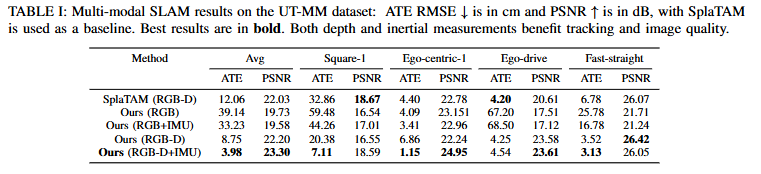
\includegraphics[width=0.8\textwidth]{Table1.png}
\caption{Multi-modal SLAM results on UT-MM dataset.}
\end{figure}

\subsection{关键发现}

\begin{itemize}
    \item \textbf{纯 RGB 效果最拉胯：} ATE 高达 39 cm，基本上没法用。原因也很明显——单目尺度模糊，又没有深度先验，光靠图像根本撑不住。
    \item \textbf{加了 IMU 之后，RGB+IMU 比纯 RGB 有明显提升：} ATE 从 39 cm 降到了 33 cm，进步是有的，但跟 RGB-D 比还是差一截。
    \item \textbf{RGB-D+IMU 组合表现最好：} ATE 做到了 3.98 cm，跟 SplaTAM \cite{SplaTAM}（12.06 cm）相比，提升了差不多 3 倍；PSNR 也涨了 5\% 左右。这个提升幅度还是挺可观的。
\end{itemize}

\subsection{我的疑问与洞察}

\paragraph{1. 为什么 RGB-D+IMU 相比纯 RGB-D，ATE 从 8.75 降到 3.98，但 PSNR 只从 22.20 涨到 23.30？}
说实话，这个差距有点意思。ATE 降了一半还多，但 PSNR 几乎没怎么动。

我的推测：IMU 主要改善的是轨迹的全局一致性，尤其是水平方向（XY 平面）的漂移。而渲染质量（PSNR）更多依赖于深度和图像的局部匹配——只要每帧的深度图足够准，局部光度误差就已经很小了，IMU 再加进来也帮不了太多。所以 PSNR 提升不大是说得通的。

\begin{figure}[H]
\centering
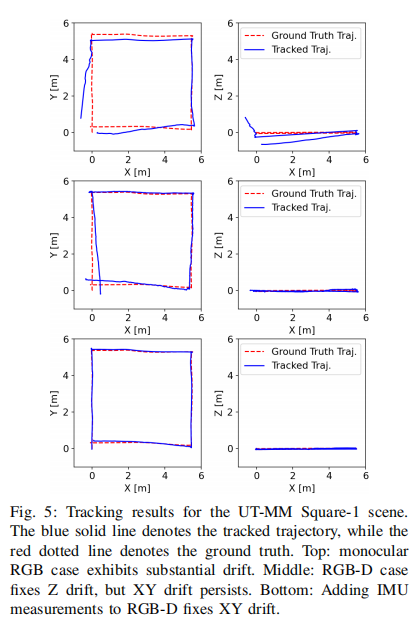
\includegraphics[width=0.75\textwidth]{table2.png}
\caption{实验截图：展示 MM3DGS 在该场景下的渲染效果。}
\end{figure}

图 5 也能印证这一点：纯 RGB-D 其实已经把 Z 方向（深度方向）的漂移消掉了，但 XY 方向的漂移还在；加上 IMU 之后，XY 漂移才被真正修正。这正好解释了为什么 ATE 降幅大而 PSNR 几乎没变——因为 PSNR 对 XY 漂移不敏感，只要每帧渲染的图和真值图看起来差不多，PSNR 就上去了。

\paragraph{2. 在 Ego-drive 场景中，为什么 RGB-D+IMU 的 ATE 反而比纯 RGB-D 还高了一点点（4.54 vs 4.25）？}
这个问题出现确实比较奇怪，可惜作者并没有解释。结合数据集的采集过程和公式，我认为可能的原因有：
\begin{itemize}
    \item 这个场景里可能有动态物体（比如行人、机动车辆），导致视觉优化本身就不太稳定，同时IMU 再给一个错误的初始估计，反而把位姿带偏了。
    \item 另一种可能是 IMU 遇到了剧烈振动，短时间内加速度或角速度饱和，开环预积分直接算出一个有偏的初值，后续视觉优化也没能完全拉回来。
\end{itemize}

从中其实也大概可以得知：惯性融合不是在所有情况下都能达到预期的效果。如果 IMU 数据质量差（饱和、振动、未标定），强行融合反而会拖后腿。一个更鲁棒的做法可能是动态调整融合权重——比如根据 IMU 的噪声方差来实时调整协方差，或者在检测到异常时自动降低 IMU 的置信度。作者在文中并没有提这个，但我觉得值得尝试一下。

\subsection{消融实验}

表 III 是在 TUM RGB-D 数据集上跑的，主要验证了两个东西的必要性：一个是 NIQE 关键帧选择，另一个是皮尔逊深度损失。结果挺有意思的。

三种配置对比：
\begin{itemize}
    \item 去掉皮尔逊损失（只靠光度） → 跟踪直接炸了，ATE 无穷大。说白了就是跑飞了，完全没法用。
    \item 保留皮尔逊损失，但不用 NIQE 关键帧 → ATE 7.81 cm，PSNR 18.05。还能跑，但精度掉了一截。
    \item 两个都用上 → ATE 5.78 cm，PSNR 18.33。虽然 PSNR 提升不大，但轨迹精度好了不少。
\end{itemize}

\section{批判性思考与未来展望}

\subsection{局限性}

\begin{itemize}
    \item \textbf{没有回环检测和全局 BA}：虽然 IMU 能减少漂移，但在长轨迹上（比如 ScanNet 里的长走廊）误差还是会慢慢累积。说实话，作者没有拿 MM3DGS 跟 GO-SLAM \cite{GO-SLAM} 或 ORB-SLAM3 \cite{ORB-SLAM3} 在长轨迹上直接对比，这是一个挺明显的短板。你回避了这个问题，那读者自然会怀疑：是不是一跑长序列就崩了？

    \item \textbf{开环 IMU 融合}：不估计偏置，意味着如果长时间没有视觉更新（比如你对着白墙或者进了黑暗房间），纯惯性积分就会飘走。作者说“短时间内的偏置误差可以被视觉优化吸收”，这话在大部分场景下没问题，但极端情况呢？万一视觉先退化，IMU 偏置已经累积起来了，后面视觉想拉也拉不回来。我觉得这个假设有点乐观。

    \item \textbf{深度估计依赖}：单目模式下用的是 DPT 网络 \cite{DPT}。这个网络在室内数据集上训练得多，拿到没见过的场景（比如户外、或者完全不同的室内风格）可能会崩。论文只在室内数据集上测了，泛化能力到底怎么样？不好说。

    \item \textbf{动态物体处理}：UT-MM 数据集里其实是有动态物体的，比如 Ego-centric-1 开始的时候有个行人走过。但论文里压根没提怎么处理动态物体。3DGS 这种显式表示很诚实——人走过的地方会留下“鬼影”高斯，如果不做任何处理，重建出来的地图里就会有一团模糊的残影。这是个问题。

    \item \textbf{计算资源}：虽然渲染能到 90 FPS，但跟踪+建图跑起来需要 RTX A5000，24GB 显存。这卡可不便宜。想在移动设备（比如无人机、手机）上跑，还有很长的路要走。
\end{itemize}

\subsection{改进思路}

\begin{itemize}
    \item \textbf{加一个轻量级回环检测}：不需要动高斯表示本身。可以借鉴 DROID-SLAM \cite{DROID-SLAM} 的帧图（frame graph）思想，在关键帧之间建立共视边，当检测到大回环时触发一个全局 BA。这个成本不大，但效果应该很明显。

    \item \textbf{把 IMU 偏置也放进局部 BA}：不要开环了，把 IMU 偏置作为优化变量加进去，联合优化视觉残差和预积分残差。ORB-SLAM3 \cite{ORB-SLAM3} 已经证明这招有效，而且增加的计算开销并不大。我觉得这是最值得加的一个模块。

    \item \textbf{加动态物体过滤}：可以用光流或者现成的语义分割（比如 Mask2Former \cite{Mask2Former}）来检测动态区域，然后把对应的高斯“静音”掉（不参与渲染和更新）。SLAM 里这类方法很成熟，直接搬过来就行。

    \item \textbf{移动端适配}：可以尝试稀疏化高斯——远处的、贡献小的高斯直接丢掉；或者用混合精度训练（FP16 甚至 INT8）。显存能降不少。
\end{itemize}

\subsection{与顶会论文的横向对比}

\begin{itemize}
    \item \textbf{对比 GO-SLAM \cite{GO-SLAM}}：GO-SLAM 虽然没 IMU，但它胜在在线回环和全局 BA，在 ScanNet 的长轨迹上跑出了 7.02 cm 的 ATE。MM3DGS 没报告长轨迹结果，所以不好直接比。但有一点是肯定的：MM3DGS 可以借鉴 GO-SLAM 的全局优化思路，把它的回环模块拿过来，效果应该会更好。

    \item \textbf{对比 ORB-SLAM3 \cite{ORB-SLAM3}}：ORB-SLAM3 的视觉-惯性紧耦合精度非常高，在 EuRoC 上 ATE 大概 3.5 cm，跟 MM3DGS 的 3.98 cm 已经很接近了。但 ORB-SLAM3 强在鲁棒性——丢了能重定位，有多地图合并。MM3DGS 呢？一旦跟踪丢了，只能重置地图，之前的全都白干。这个差距还是挺大的。说白了，MM3DGS 目前还比较理想化，离实际应用还有一定距离，不像 ORB-SLAM3 那么皮实。
\end{itemize}

\subsection{未来可延伸的研究问题}

\begin{itemize}
    \item \textbf{生成式高斯 SLAM}：我在想能不能将 3DGS 和扩散模型结合起来？比如当其看到一半的场景，让模型“脑补”出没看到的部分，这样地图会更完整。当然，这样生成的地图可能不准，但如果做 AR/VR 的时候也许够用。

    \item \textbf{事件相机 + IMU + 3DGS}：因为事件相机动态范围大、延迟低，所以我在想可不可以配合 IMU 可以挑战极端高速运动（比如无人机急速翻滚）。3DGS 的快速渲染正好能跟上。这个方向我觉得值得尝试一下。

    \item \textbf{无监督深度估计与 SLAM 联合训练}：现在的 DPT \cite{DPT} 是固定死的。如果把它跟 SLAM 放在一起联合微调，让深度网络适应当前场景，精度可能还能再提一截。不过训练起来会比较麻烦，而且可能过拟合。
\end{itemize}

\begin{thebibliography}{99}
\bibitem{MM3DGS}
Sun, L. C., Bhatt, N. P., Liu, J. C., Fan, Z., Wang, Z., Humphreys, T. E., \& Topcu, U. (2024).
\newblock MM3DGS SLAM: Multi-modal 3D Gaussian splatting for SLAM using vision, depth, and inertial measurements.
\newblock \emph{arXiv preprint arXiv:2404.00923}.

\bibitem{DROID-SLAM}
Teed, Z., \& Deng, J. (2021).
\newblock DROID-SLAM: Deep Visual SLAM for Monocular, Stereo, and RGB-D Cameras.
\newblock \emph{arXiv preprint arXiv:2108.10869}.

\bibitem{SplaTAM}
Keetha, N., Karhade, J., Jatavallabhula, K. M., Yang, G., Scherer, S., Ramanan, D., \& Luiten, J. (2024).
\newblock SplaTAM: Splat, track \& map 3D Gaussians for dense RGB-D SLAM.
\newblock \emph{arXiv preprint arXiv:2312.02126}.

\bibitem{GO-SLAM}
Zhang, Y., Tosi, F., Mattoccia, S., \& Poggi, M. (2023).
\newblock GO-SLAM: Global optimization for consistent 3D instant reconstruction.
\newblock \emph{arXiv preprint arXiv:2309.02436}.

\bibitem{ORB-SLAM3}
Campos, C., Elvira, R., Gómez Rodríguez, J. J., Montiel, J. M. M., \& Tardós, J. D. (2021).
\newblock ORB-SLAM3: An accurate open-source library for visual, visual-inertial and multi-map SLAM.
\newblock \emph{arXiv preprint arXiv:2007.11898}.

\bibitem{DPT}
Ranftl, R., Bochkovskiy, A., \& Koltun, V. (2021).
\newblock Vision Transformers for Dense Prediction.
\newblock \emph{arXiv preprint arXiv:2103.13413}.

\bibitem{Mittal2013}
Mittal, A., Soundararajan, R., \& Bovik, A. C. (2013).
\newblock Making a ``Completely Blind'' Image Quality Analyzer.
\newblock \emph{IEEE Signal Processing Letters}, 20(3), 209--212.

\bibitem{Mask2Former}
Cheng, B., Misra, I., Schwing, A. G., Kirillov, A., \& Girdhar, R. (2022).
\newblock Masked-attention Mask Transformer for Universal Image Segmentation.
\newblock In \emph{Proceedings of the IEEE/CVF Conference on Computer Vision and Pattern Recognition (CVPR)}.

\end{thebibliography}

\end{document}